\documentclass{report}

\usepackage{textcomp}
\usepackage{graphicx}
\usepackage{fancyhdr}
\usepackage{subcaption}
\usepackage{multicol}
\usepackage{outlines}
%===================================
\newcommand{\classinfo}{{\bf Configuring DHCP IPv4 \\ Using Cisco IOS}\\{\it CIT 167}\\{Chaz Davis}}
\newcommand{\semester}{BCTC \\ Spring 2020}
%===================================
\newcommand{\mysection}[1]{\section*{#1}}
\newcommand{\mysubsection}[2]{\textbf{\romannumeral #1) #2}}
%===================================
\setlength{\headheight}{15.2pt}
\pagestyle{fancy}
\fancyhf{}
\lhead{ \fancyplain{}{Chaz Davis} }
\rhead{ \fancyplain{}{\today} }
\cfoot{ \fancyplain{}{\thepage} }
\renewcommand{\headrulewidth}{0.5pt}
\renewcommand{\footrulewidth}{0pt}

%===================================
\title{\classinfo}
\author{\semester}
\date{\today}

%===================================

\begin{document}

\maketitle

%===================================
\mysection{\textbf{Part 1: Configure a Router as a DHCP Server}}

\mysubsection{1}{Configure the excluded addresses}\\
I ran logged into R2, went to global configuration, and ran 
{\scriptsize{\verb$ip dhcp excluded-address$}} 
{\scriptsize{\verb$192.168.10.1 192.168.10.10$}\normalsize} 
to block off the lowest 10 address on the R1 network. I then ran 
{\scriptsize{\verb$ip dhcp excluded-address$}\normalsize} 
{\scriptsize{\verb$192.168.30.1 192.168.30.10$}\normalsize} 
to block off the lowest 10 addresses on the R3. See
Fig.~\ref{P1Config19}\subref{P1Config19Exc}.


\noindent\mysubsection{2}{Create a DHCP pool on R2 for the R1 LAN}\\
I created dhcp pools by going to gloabal config, and typing
{\scriptsize{\verb$ip dhcp pool R1-LAN$}\normalsize}. 
I set the network, default-router, and dns-server.
See Fig.~\ref{P1Config19}\subref{P1Config19R1} for R1-LAN configuration.

\noindent\mysubsection{3}{Create a DHCP pool on R2 for the R3 LAN}\\
a
I created the dhcp pool for R3 by going to gloabl config for R2, and typing
{\scriptsize{\verb$ip dhcp pool R3-LAN$}\normalsize}. I then configured the
network, default-router, and dns-server.
See Fig.~\ref{P1Config19}\subref{P1Config19R3} for R3-LAN configuration.


\begin{figure}[!hbt]\centering
\subfloat[Creating the excluded addresses]{\label{P1Config19Exc}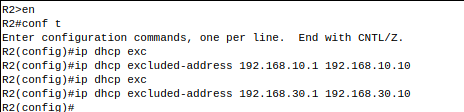
\includegraphics[width=.45\linewidth]{Figures/P1/2020-03-26-205348_464x112_scrot.png}}\par
\subfloat[Configuring R1-LAN]{\label{P1Config19R1}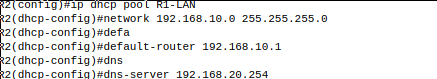
\includegraphics[width=.45\linewidth]{Figures/P1/2020-03-26-205726_437x79_scrot.png}}\hfill
\subfloat[Configuring R3-LAN]{\label{P1Config19R3}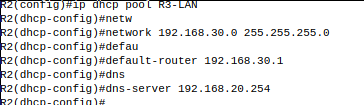
\includegraphics[width=.45\linewidth]{Figures/P1/2020-03-26-205736_364x105_scrot.png}}\par
\caption{Configurations for Part 1}\label{P1Config19}
\end{figure}

%===================================
\mysection{\textbf{Part 2: Configure DHCP Relay}}

\mysubsection{1}{Configure R1 and R3 as a DHCP relay agent}\\
I went to R1 and R3, went into Global configurations and went to Interface G0/0
on each. For R1 I ran
{\scriptsize{\verb$ip dhcp helper-address 10.1.1.2$}\normalsize}
(Fig.~\ref{P2Config19}\subref{P2Config19R1}), because that was the address for
the interface s0/0/0 connecting to R2. For R3 I ran the command
{\scriptsize{\verb$ip helper-address 10.2.2.2$}\normalsize}
(Fig.~\ref{P2Config19}\subref{P2Config19R3}), because that was the address
connecting R3 to R2 on the s0/0/1 interface.

\noindent\mysubsection{2}{Set PC1 and PC2 to recieve IP addressing information
from DHCP}\\
I went into the Ip configuration for PC-1 and PC-2 and set their IPv4
addressing to come from DHCP, and allowed them to gain access from the server.
See Fig.~\ref{P2Config19}\subref{P2Config19PC1} and
Fig.~\ref{P2Config19}\subref{P2Config19PC2}.


\begin{figure}[!hbt]\centering
\subfloat[Configuring R1 as a DHCP agent]{\label{P2Config19R1}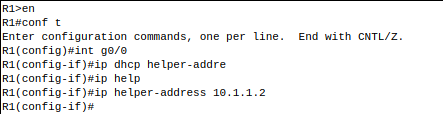
\includegraphics[width=.45\linewidth]{Figures/P2/2020-03-26-210132_443x114_scrot.png}}\hfill
\subfloat[Configuring R3 as a DHCP agent]{\label{P2Config19R3}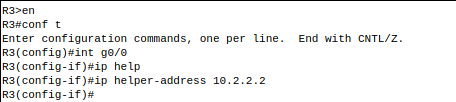
\includegraphics[width=.45\linewidth]{Figures/P2/2020-03-26-210142_456x102_scrot.png}}\par
\subfloat[Configuring And applying DHCP addressing to PC-1]{\label{P2Config19PC1}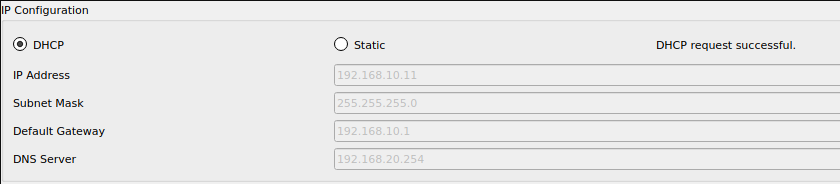
\includegraphics[width=.45\linewidth]{Figures/P2/2020-03-26-210252_840x184_scrot.png}}\hfill
\subfloat[Configuring and applying DHCP addressing to PC-2]{\label{P2Config19PC2}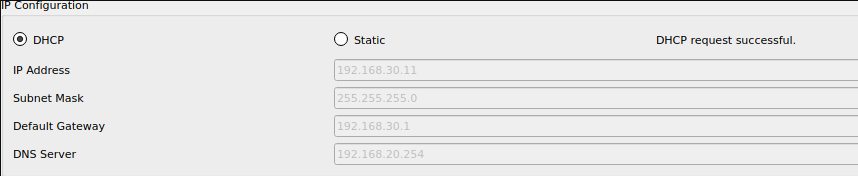
\includegraphics[width=.45\linewidth]{Figures/P2/2020-03-26-210306_858x176_scrot.png}}\par
\caption{Configuring DHCP Relay}\label{P2Config19}
\end{figure}

%===================================
\mysection{\textbf{Part 3: Configure R2 as a DHCP Client}}
I went in to global config mode on R2, and configured interface G0/1 for DHCP by
running the command
{\scriptsize{\verb$ip address dhcp$}\normalsize} and then 
{\scriptsize{\verb$no shut$}\normalsize}. See Fig.~\ref{P3Config19}.


\begin{figure}[!hbt]\centering
\subfloat[Configuring G0/0 for DHCP]{\label{P3Config19a}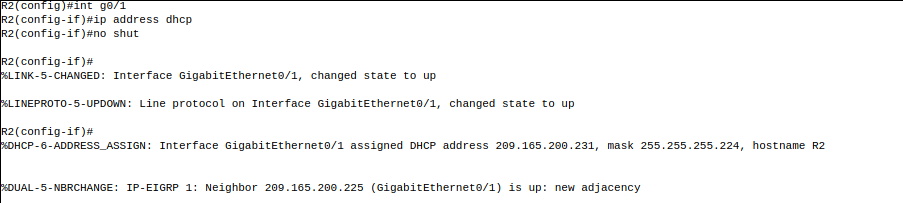
\includegraphics[width=.45\linewidth]{Figures/P3/2020-03-26-210540_903x203_scrot.png}}\hfill
\subfloat[G0/0 show ip int brief]{\label{P3Config19b}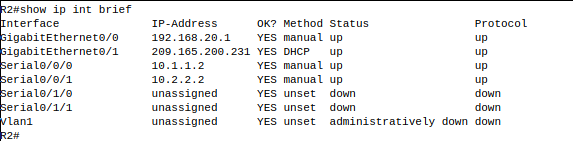
\includegraphics[width=.45\linewidth]{Figures/P3/2020-03-26-210631_573x141_scrot.png}}\par 
\caption{Configuring R2 as a DHCP client}\label{P3Config19}
\end{figure}

%===================================
\mysection{\textbf{Part 4: Verify DHCP and Connectivity}}
\mysubsection{1}{Verify DHCP Bindings}\\
The output of the {\scriptsize{\verb$show ip dhcp bindings$}\normalsize} on R2
is shown in Fig.~\ref{P4Config19}


\begin{figure}[!h]
    \centering
    {\label{P4Config19}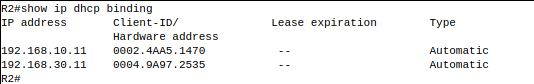
\includegraphics[width=.45\linewidth]{Figures/P4/2020-03-26-210759_534x84_scrot.png}}
  \caption{Verifying the DHCP Bindings on R2}
\end{figure}

\noindent\mysubsection{2}{Verifying Configurations}\\
You Can see the output of PC-1 pinging, PC-2, the DHCP server, and the cisco
website in Fig.~\ref{P4Verify19}\subref{P4Verify19PC1}. You can see the output of
PC-2 pinging PC-1, the DHCP server, and the cisco website in
Fig.~\ref{P4Verify19}\subref{P4Verify19PC2}.


\begin{figure}[!hbt]\centering
\subfloat[PC-1 Pinging the Network and web]{\label{P4Verify19PC1}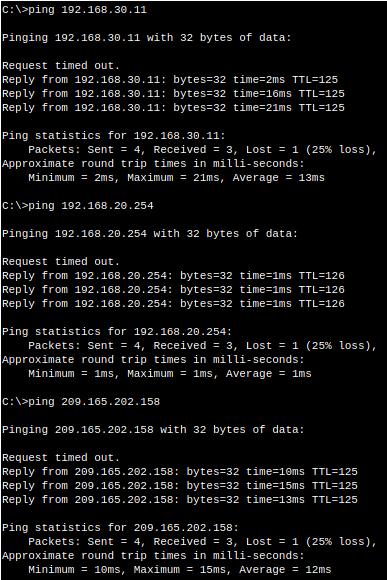
\includegraphics[width=.45\linewidth]{Figures/P4/2020-03-26-211315_387x580_scrot.png}}\hfill
\subfloat[PC-2 Pinging the network and web]{\label{P4Verify19PC2}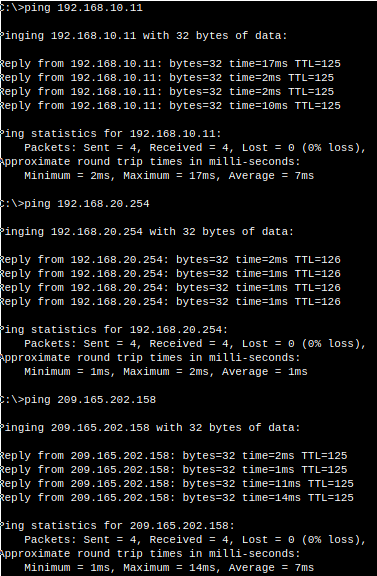
\includegraphics[width=.45\linewidth]{Figures/P4/2020-03-26-211335_377x576_scrot.png}}\par 
\caption{Confirming the configuration of the network}\label{P4Verify19}
\end{figure}


\noindent\mysubsection{3}{The End Verified}\\


\begin{figure}[!hbt]\centering
\subfloat[Complete]{\label{Complete19a}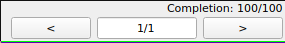
\includegraphics[width=.45\linewidth]{Figures/P4/2020-03-26-211406_285x43_scrot.png}}\hfill
\subfloat[Complete]{\label{Complete19b}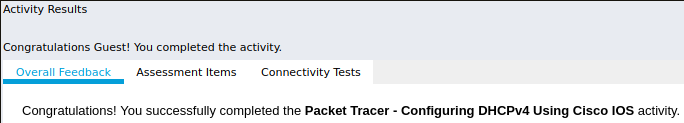
\includegraphics[width=.45\linewidth]{Figures/P4/2020-03-26-211425_684x123_scrot.png}}\par 
\subfloat[Complete]{\label{Complete19c}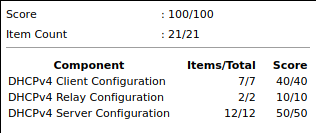
\includegraphics[width=.45\linewidth]{Figures/P4/2020-03-26-211451_316x133_scrot.png}}
\caption{The end complete}\label{Complete19}
\end{figure}



%===================================

\end{document}
